% THIS IS A LATEX TEMPLATE FILE FOR PAPERS INCLUDED IN THE
% *Anthology of Computers and the Humanities*. ADD THE OPTION
% 'final' WHEN CREATING THE FINAL VERSION OF THE PAPER. 
% DO NOT change the documentclass
%\documentclass[final]{anthology-ch} % for the final version
\documentclass{anthology-ch}         % for the submission

% LOAD LaTeX PACKAGES
\usepackage{booktabs}
\usepackage{graphicx}
% ADD your own packages using \usepackage{}
%\usepackage[style=chicago-authordate,backend=biber]{biblatex}
\addbibresource{references.bib}

% TITLE OF THE SUBMISSION
% Change this to the name of your submission
\title{Neutral Drift and Cumulative Memory:\\
A Wright--Fisher Model of Thematic Evolution\\
in Online Horror Fiction}

% AUTHOR AND AFFILIATION INFORMATION
% For each author, include a new call to the \author command, with
% the numbers in brackets indicating the associated affiliations 
% (next section) and ORCID-ID for each author.  
\author[1,3]{Alexandre Lionnet}[
  orcid=0009-0002-1131-8447
]

\author[2,3]{Florian Cafiero}[
  orcid=0000-0002-1951-6942
]

% While we encourage including ORCID-IDs for all authors, you can
% include authors that do not have one by definining an empty ID.


% There should be one call to \affiliation for each affiliation of
% the authors. Multiple affiliations can be given to each author
% and an affiliation can be given to multiple authors. 
\affiliation{1}{École Pratique des Hautes Études -- PSL, Paris}
\affiliation{2}{École Nationale des Chartes -- PSL, Paris}
\affiliation{3}{Centre Jean Mabillon, Paris}

% KEYWORDS
% Provide one or more keywords or key phrases seperated by commas
% using the following command
\keywords[eng]{Online Literature, cultural evolution, modelling, creepypasta, internet}

% METADATA FOR THE PUBLICATION
% This will be filled in when the document is published; the values can
% be kept as their defaults when the file is submitted
\pubyear{2025}
\pubvolume{1}
\pagestart{1}
\pageend{1}
\paperorder{1}
\conferencename{Proceedings of Conference XXX}
\conferenceeditors{Editor1 Editor2}
\doi{00000/00000}  
\customhead{}  



%%%%%%%%%%%%%%%%%%%%%%%%%%%%%%%%%%%%%%%%%%%%%%%%%%%%%%%%%%%%%%%%%%%%%%%%%%%
% HERE IS THE START OF THE TEXT
\begin{document}

\maketitle

\begin{abstract}
Cultural evolutionary models offer a principled framework for understanding how digital genres stabilise over time. In this paper, we apply a modified Wright--Fisher model to the thematic evolution of creepypasta narratives published on the Creepypasta Fandom wiki between 2010 and 2024.
Drawing on a corpus of 13,128 stories tagged across 176 moderated thematic categories, we test whether the observed power-law distribution of themes can be reproduced by a neutral drift process augmented with cumulative archiving. 
Standard Wright--Fisher simulations fail to replicate the empirical long tail, as minor categories extinguish too rapidly. When a mechanism of cumulative memory is introduced---whereby each generation contributes a sampled archive that persists alongside the living population---the model successfully reproduces both the dominance of major themes and the stable persistence of rare ones. 
Maximum-likelihood fitting confirms that both the empirical distribution and the simulated archive follow a power law with comparable exponents, supporting the qualitative agreement between model and data. These results suggest that the thematic structure of the Fandom corpus is best understood not as a snapshot of active production, but as a sedimented historical record whose composition reflects processes of neutral drift operating over a cumulative substrate. We discuss implications for platform studies and the modelling of digital literary evolution.
\end{abstract}

\section{Introduction} 

The question of how genres stabilise has long been central to literary sociology \cite{guillory1993cultural}. In the case of print literature, stabilisation is typically attributed to the action of mediating institutions---publishers, critics, university curricula---which select, amplify, and canonise certain formal and thematic configurations while allowing others to disappear \cite{moretti2000slaughterhouse}. 
The rise of born-digital vernacular genres, however, challenges this institutional model: on platforms such as Reddit or dedicated fandom wikis, thousands of authors publish without editors or commercial gatekeepers, yet recognisable and stable genre structures nonetheless emerge \cite{howard2008networked, blank_folklore_2009}.


Creepypasta---short user-generated horror narratives that originally circulated through copy-paste practices on imageboards and forums---constitutes a particularly apt case for studying bottom-up genre stabilisation. Its ecology is now distributed across heterogeneous platforms: Reddit's \texttt{/r/nosleep}, the Creepypasta Fandom wiki, and dedicated archival sites each host distinct populations of stories under varying rule regimes. 
Previous work has shown that canonical status within this ecosystem is predicted by stylistic rather than affective features, and that platform-specific rules exert surprisingly little influence on surface-level prose style . \cite{lionnet2025makes}
What remains unexplored is the \emph{thematic} dimension: how do the topics around which creepypasta organises itself distribute and persist over time?

Cultural evolutionary theory offers a productive framework for addressing this question. Foundational work in this tradition demonstrated that cultural transmission can be modelled using mechanisms borrowed from population genetics \cite{boyd1988culture}, and subsequent studies have applied such models to the survival of manuscripts \cite{Weitzman1987}, the extinction of textual traditions \cite{kestemont2022forgotten}, and the dynamics of linguistic change \cite{blythe2007stochastic, acerbi2023individual}. Within this framework, themes function as discrete, transmissible units---analogous to alleles---that can be extracted from one narrative and reinjected into another, independently of surface form. Their distribution across a corpus at a given moment thus constitutes an evolutionary snapshot amenable to formal modelling.

The present paper develops this intuition. We ask whether the empirically observed thematic distribution of a large creepypasta corpus can be reproduced by a neutral drift model, and what modifications to the standard framework are required to achieve a satisfactory fit. Our central finding is that a cumulative archiving mechanism---representing the platform's tendency to retain rather than replace older content---is sufficient to replicate the observed power-law structure, including the stable persistence of low-frequency themes that standard Wright--Fisher dynamics would rapidly eliminate. Power-law distributions are ubiquitous in cultural diffusion phenomena and can arise from a variety of mechanisms \cite{newman2006power, simkin2010re}; our claim is not that cumulative archiving is the unique generative process, but that it provides a parsimonious and empirically adequate account of this particular corpus.


\section{Data and Methods}

\subsection{Data Collection \& Overview}

Stories were collected from the Creepypasta Fandom wiki\footnote{\url{https://creepypasta.fandom.com/wiki/Creepypasta_Wiki}} using a two-stage scraping pipeline. The site's architecture departs from a conventional tree structure: rather than organising content hierarchically, pages are linked laterally around a small number of central reference pages. This organisation precludes exhaustive crawling strategies based on site structure, as no canonical entry point indexes the full corpus from the homepage. Instead, navigation depends on following hyperlinks between pages, with a single reference page---not directly accessible from the homepage---serving as the practical gateway to the complete story catalogue.

In the first stage, all story URLs were extracted by iterating through the paginated reference index. Selenium was used to simulate user navigation, including successive clicks on the \emph{next page} button, while BeautifulSoup parsed the resulting HTML to collect individual page links. In the second stage, each story page was fetched and its relevant elements extracted: the narrative body and the associated tags that act as thematic categories. In this work, we solely focus on the thematic categories.



%\begin{table}[h]
%\centering
%\caption{Token-length statistics for the Creepypasta Fandom corpus.}
%\label{tab:corpus_stats}
%\resizebox{\textwidth}{!}{%
%\begin{tabular}{lrrrrrrrrr}
%\toprule
%Source & $n$ & Mean & SD & Min & Q1 & Median & Q3 & Max \\
%\midrule
%Fandom & 11{,}379 & 2{,}095.9 & 5{,}147.0 & 1 & 637.5 & 1{,}201.0 & 2{,}259.5 & 257{,}078 \\
%\bottomrule
%\end{tabular}
%}
%\end{table}


\subsection{Thematic Categorisation}

The Creepypasta Fandom wiki organises its content through a moderated tagging system. At the time of data collection, 176 thematic categories were in active use across a corpus of 13,128 stories. Each story may carry multiple tags, yielding a total of 30,901 theme occurrences---a figure substantially higher than the document count, which must be borne in mind when interpreting distributional statistics.

Moderation provides a key methodological advantage over freely assigned tags: the vocabulary of categories is controlled and consistent across the corpus, reducing the terminological drift typical of user-generated classification systems.

This infrastructure guarantees sufficient coherence for the distributional analysis and subsequent modelling.

\subsection{Exploratory Analysis}

Before modelling, we characterise the empirical distribution of thematic categories. For each of the 176 categories, we compute the number of associated documents and examine the resulting frequency spectrum. We additionally track the temporal evolution of category frequencies across the full span of the corpus (2010--2024) in order to identify phases of growth and stabilisation.

\subsection{The Wright--Fisher Model and its Extensions}

\subsubsection{Standard Multi-class Framework}

The Wright--Fisher model is a foundational framework in population genetics describing the evolution of trait frequencies in a finite population under neutral drift \cite{fisher1999genetical, wright1931evolution}. In its classical formulation, a population of fixed size $N$ is renewed at each discrete generation by random sampling with replacement from the previous generation.

For a two-allele system, the count $X^{(t+1)}$ of allele $A$ in the next generation follows:

\begin{equation}
X^{(t+1)} \sim \text{Binomial}\!\left(N,\, p^{(t)}\right)
\end{equation}

where $p^{(t)} = X^{(t)}/N$ is the current frequency of $A$. This process is extended here to $n$ thematic classes $C = \{0, 1, \ldots, n-1\}$. Each individual $i \in \{1,\ldots,N\}$ carries a class label $c_i^{(t)} \in C$ at generation $t$. The class of individual $i$ in the next generation is drawn by uniform sampling from the current population:

\begin{equation}
c_i^{(t+1)} \sim \text{Uniform}\!\left\{c_1^{(t)}, c_2^{(t)}, \ldots, c_N^{(t)}\right\}, \quad i = 1, \ldots, N
\end{equation}

The count of individuals belonging to class $k$ at generation $t$ is denoted $n_k^{(t)} = \#\{i : c_i^{(t)} = k\}$, and its frequency $p_k^{(t)} = n_k^{(t)}/N$.

\subsubsection{Population Growth}

To reflect the empirically observed growth in platform content, we allow the active population size $N(t)$ to increase linearly over $T_{\max}$ generations from an initial size $n_i$ to a final size $n_f$. Note that this growth is maintained in the cumulative archiving version of the model: $N(t)$ describes the active production dynamics, while the observable corpus is tracked separately by $\mathcal{A}_{\mathrm{cum}}(t)$.

\begin{equation}
N(t) = \left\lfloor n_i + t \cdot \frac{n_f - n_i}{T_{\max}} \right\rfloor
\end{equation}

\subsubsection{Cumulative Archiving}

The key modification introduced in this paper is a mechanism of cumulative archiving. At each generation $t$, a fraction $\alpha \in [0,1]$ of the active population is sampled without replacement and permanently added to an archive $\mathcal{A}(t)$ of size $M(t) = \lfloor \alpha \cdot N(t) \rfloor$. The cumulative archive aggregates all past samples:

\begin{equation}
\mathcal{A}_{\mathrm{cum}}(t) = \bigcup_{\tau=0}^{t} \mathcal{A}(\tau), \qquad \left|\mathcal{A}_{\mathrm{cum}}(t)\right| = \sum_{\tau=0}^{t} M(\tau)
\end{equation}

For each class $c \in C$, the proportion of that class in the cumulative archive at time $t$ is:

\begin{equation}
p_c(t) = \frac{n_c(t)}{\left|\mathcal{A}_{\mathrm{cum}}(t)\right|}
\end{equation}

where $n_c(t)$ is the total count of archived individuals of class $c$ up to $t$. It is this quantity---not the active population frequency---that we compare to empirical data, on the grounds that the platform corpus is itself a cumulative archive rather than a living, self-renewing population.

\subsubsection{Parameters}

Simulations were run with the following parameters: $n = 40$ thematic classes, initial population $n_i = 1{,}000$, final population $n_f = 2{,}000$, $T = 1{,}000$ total generations, and analysis window $[0, t]$ with $t = 300$. Two initialisation conditions were tested: uniform random assignment of classes, and a power-law initial distribution matching the empirical dominance structure. Archive fraction $\alpha = 0.05$ was used, meaning 5\% of the active population is sampled at each generation and permanently added to the archive. It is worth noting that $n_i$, $n_f$, and $\alpha$ are not fully independent: rescaling all three by a common factor leaves the growth trajectory of the cumulative archive unchanged, so one parameter can in principle be fixed by external considerations such as the observed ratio of cumulative to active content on the platform.


\section{Results}

\subsection{Empirical Distribution of Themes}

The empirical distribution of thematic categories is highly skewed. The single most frequent category---\emph{Beings}---is associated with 3,158 documents, representing nearly 10\% of all theme occurrences. It is followed by \emph{Mental Illness} (2,698 occurrences, 8.7\%), \emph{Places} (1,688), \emph{Reality} (1,269), and \emph{Dismemberment} (1,263). The dominance of \emph{Beings} and \emph{Places} aligns with evolutionary accounts of horror \cite{clasen2017}, as these categories engage ancestral predator-detection and environmental vigilance mechanisms; similarly, the high frequency of \emph{Mental Illness} and \emph{Dismemberment} targets evolved fears of unpredictable conspecifics and pathogen-related disgust. Together, the top five categories account for over a third of all tag assignments; at the opposite extreme, 26 categories appear only once. When examined on a logarithmic scale, the full distribution follows a power law: a tiny number of categories dominate while the vast majority are associated with only a handful of documents (Figure~\ref{fig:log_log}). This distributional shape is reminiscent of preferential attachment, but the mechanism explored here is distinct: sampling is strictly uniform, with no built-in bias toward larger classes, and the skewed distribution emerges from stochastic drift combined with cumulative memory.


\begin{figure}[htbp]
    \centering
    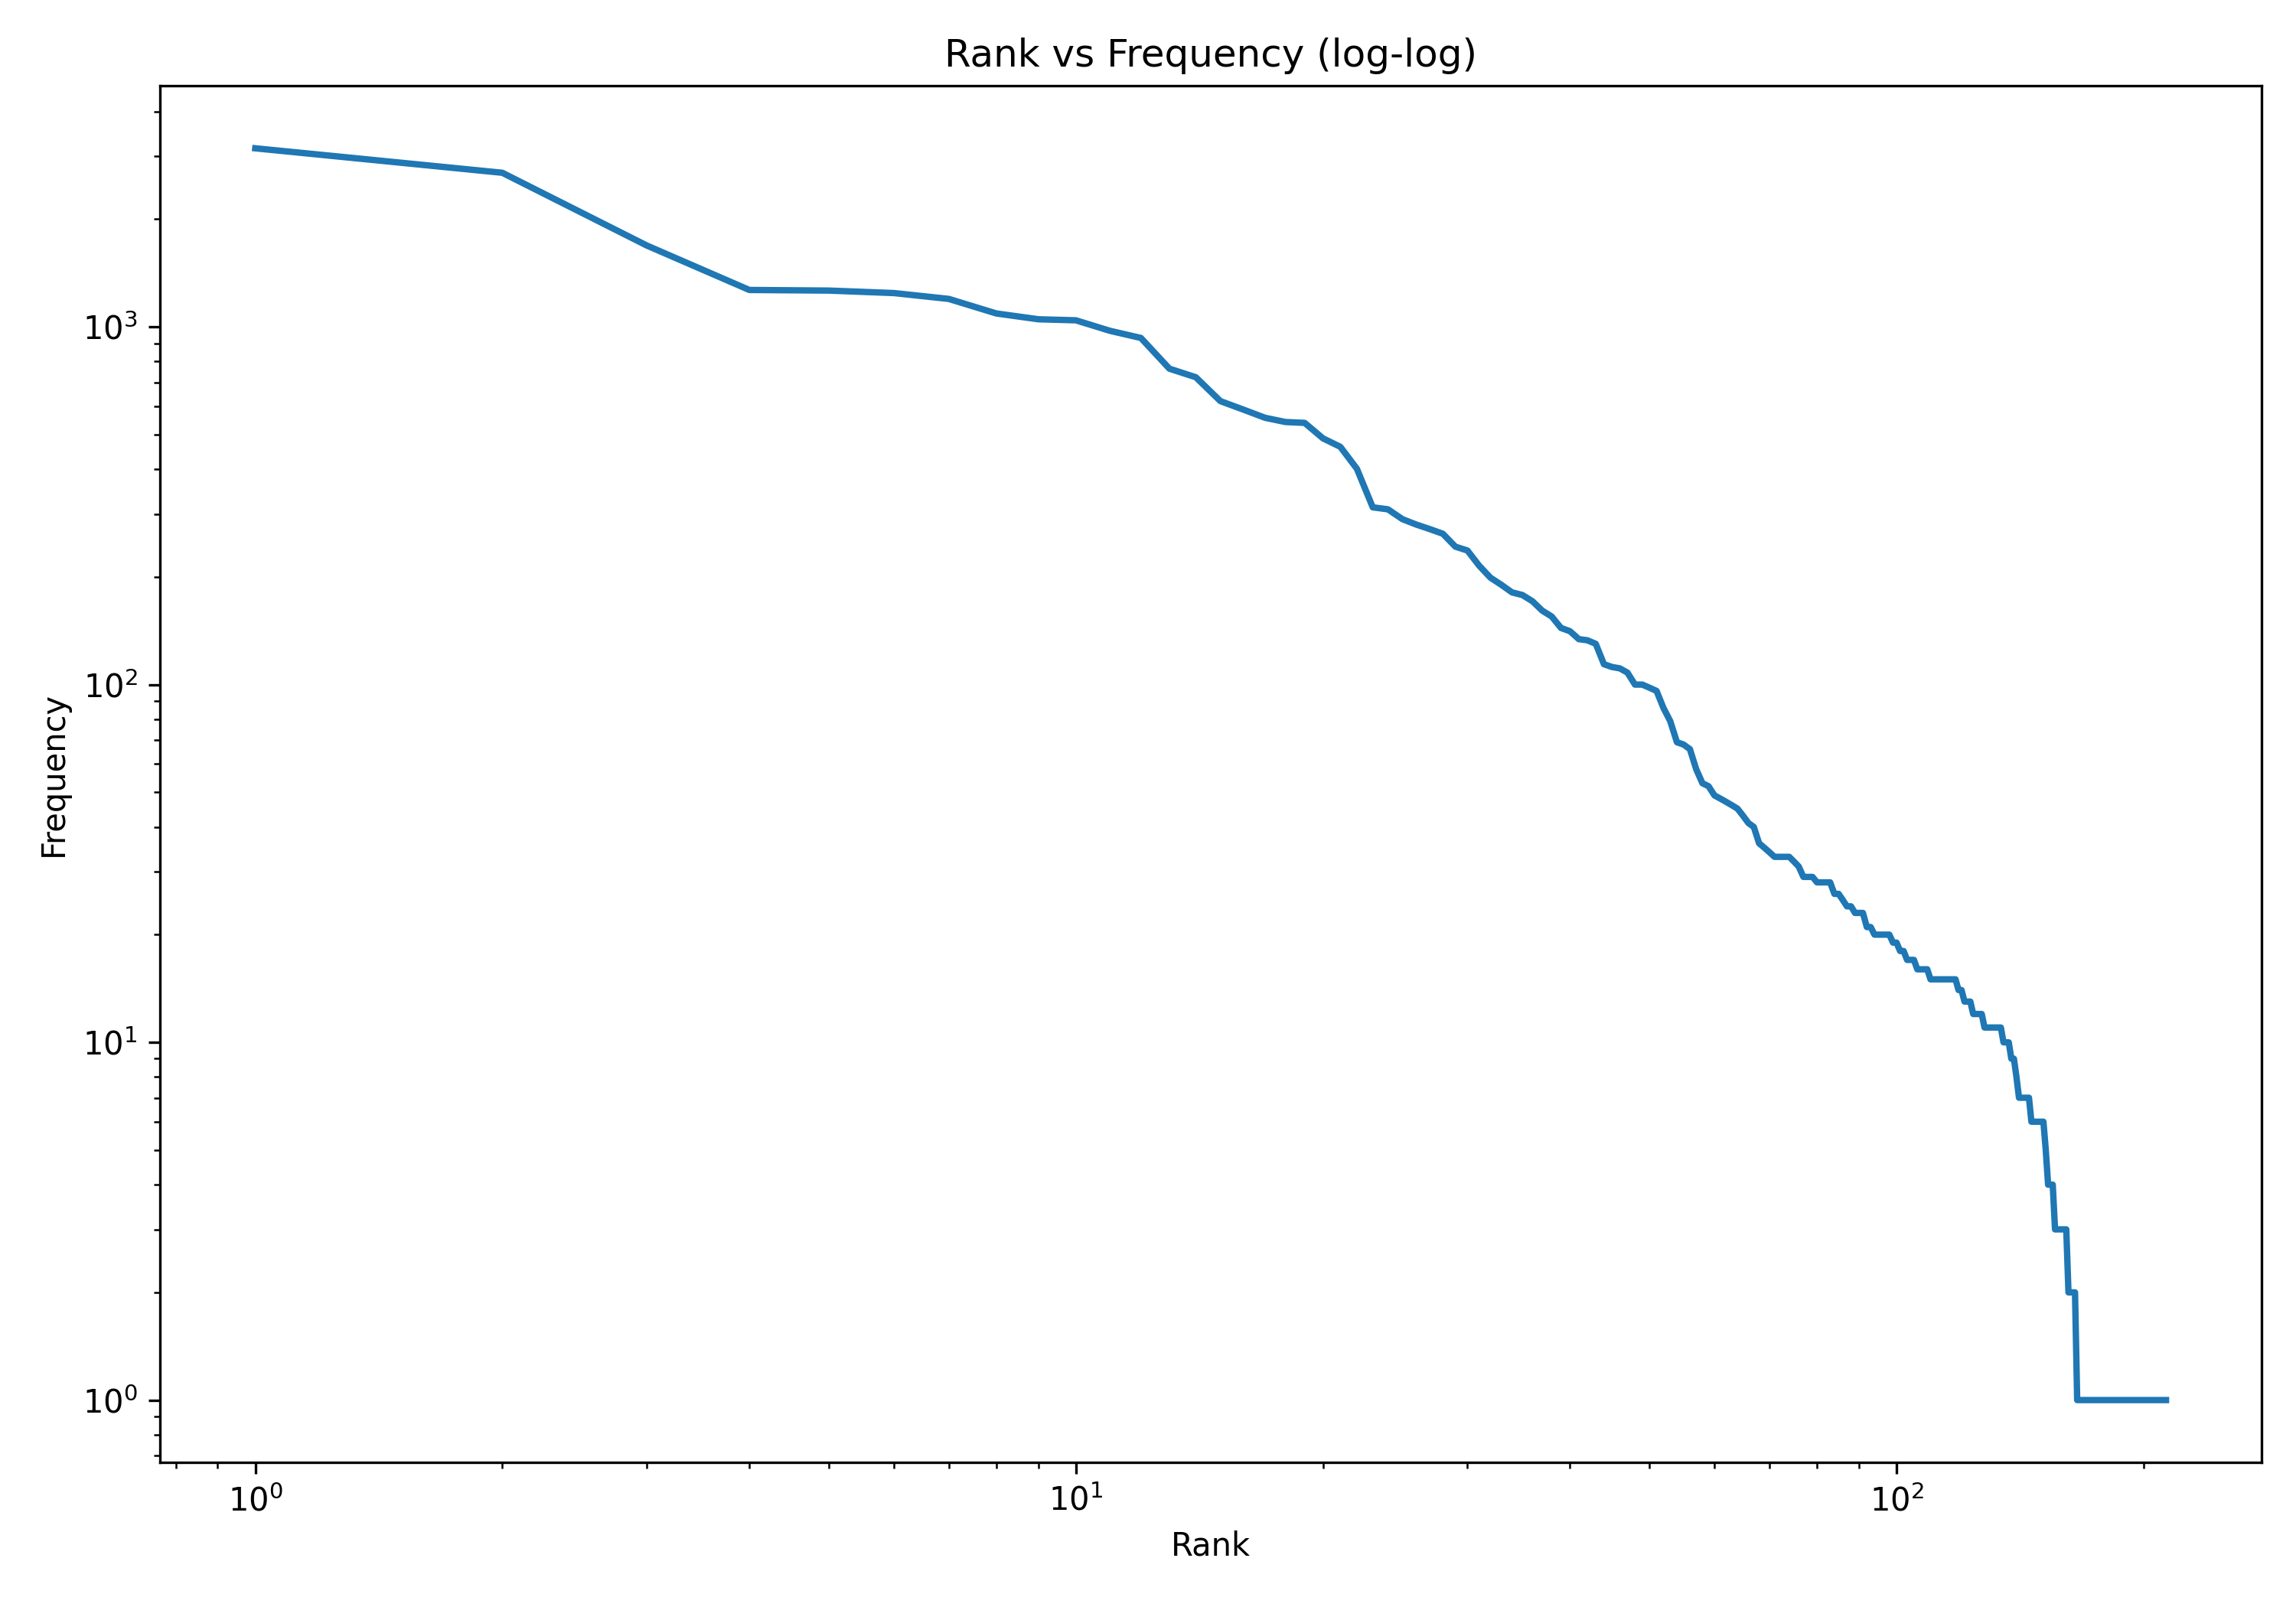
\includegraphics[width=\textwidth]{illustration/zipf_loglog.png}
    \caption{Log-log rank--frequency distribution of thematic categories (empirical data, ranked by frequency at time of collection)}
    \label{fig:log_log}
\end{figure}

\begin{figure}[htbp]
    \centering
    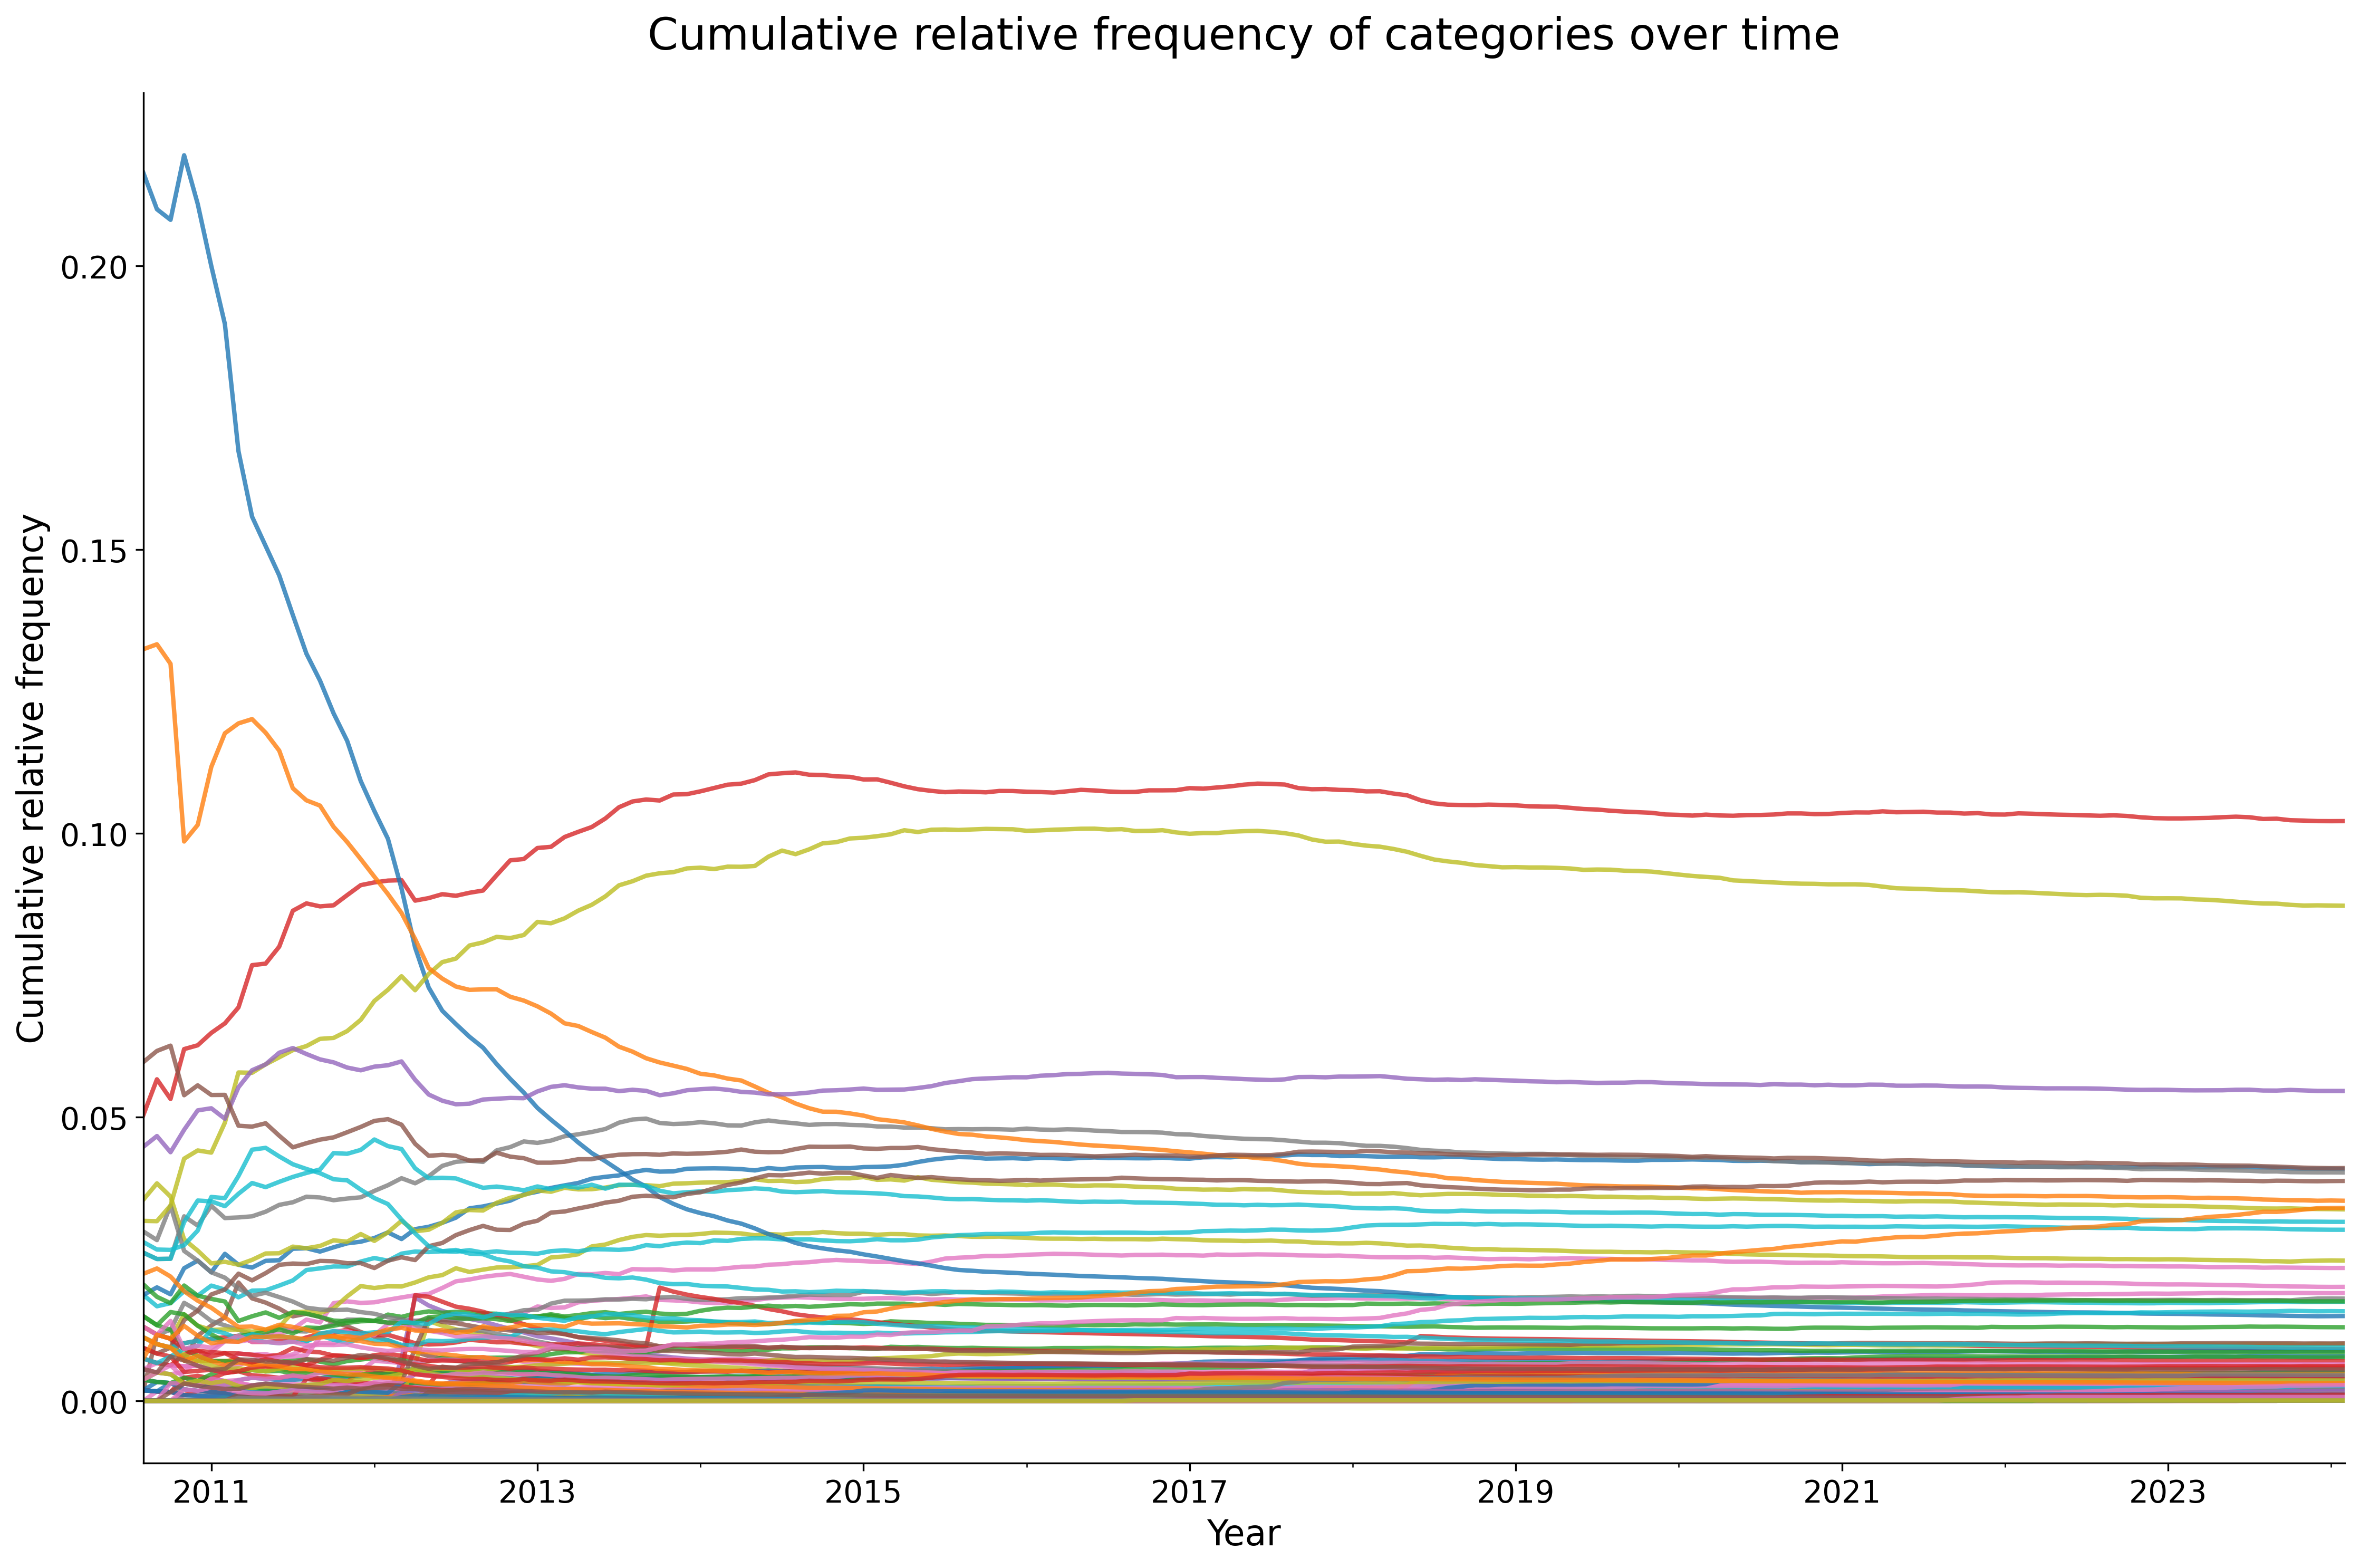
\includegraphics[width=\textwidth]{illustration/cumulative_relative_frequency.png}
    \caption{Relative frequency of thematic categories over time (empirical data, 2010--2024)}
    \label{fig:freq_relative_cat}
\end{figure}

Temporal analysis reveals two distinct phases. Between 2010 and approximately 2015, both production volume and the relative frequencies of individual categories evolve substantially. From 2015 onward, relative category proportions stabilise despite continued publication activity (Figure~\ref{fig:freq_relative_cat}). This freeze is interpreted as evidence that the corpus represents a historical accumulation whose compositional structure was largely determined during the early growth phase, rather than an active, continuously self-renewing population.

Two factors plausibly account for this transition. First, the emergence and growing popularity of Reddit's \texttt{/r/nosleep} around 2015 likely diverted creative output away from the Fandom platform, reducing the rate of thematically novel contributions. Second, concurrent shifts in content consumption habits---notably the rise of smartphone-first browsing favouring dedicated applications---may have further accelerated this audience transfer. In the absence of direct traffic data, however, we treat these interpretations as provisional.

\subsection{Baseline Wright--Fisher Simulations}

Standard Wright--Fisher simulations, whether initialised with a uniform or a power-law distribution, fail to reproduce the empirical thematic structure. Under both conditions, minor categories extinguish rapidly: the model converges toward a monocultural state in which only a handful of alleles survive (Figure~\ref{fig:wf_vanilla}). Initialisation from a power-law distribution preserves the short-term dominance of major classes but accelerates the loss of minor ones relative to the random-start condition, producing an even poorer fit to the observed long tail (Figure~\ref{fig:wf_power}). The baseline model is thus insufficient: its fundamental absence of memory causes the system to forget its past compositional diversity far more quickly than the empirical corpus.

\begin{figure}[htbp]
    \centering
    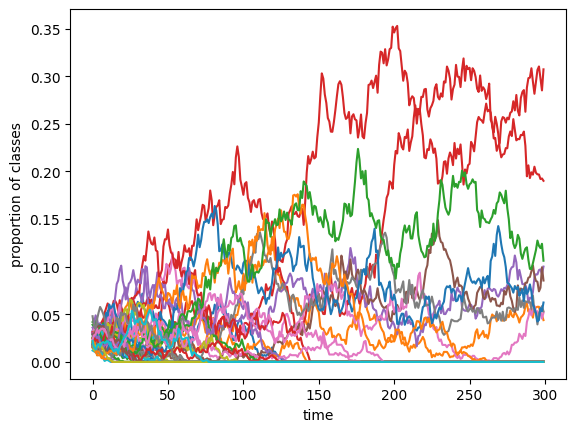
\includegraphics[width=\textwidth]{illustration/wf_vanilla.png}
    \caption{Standard multi-class Wright--Fisher model, uniform initialisation ($n=40$, $n_i=1{,}000$, $n_f=2{,}000$, $T=1{,}000$). Class proportions in the active population over $t \in [0, 300]$.}
    \label{fig:wf_vanilla}
\end{figure}


\begin{figure}[htbp]
    \centering
    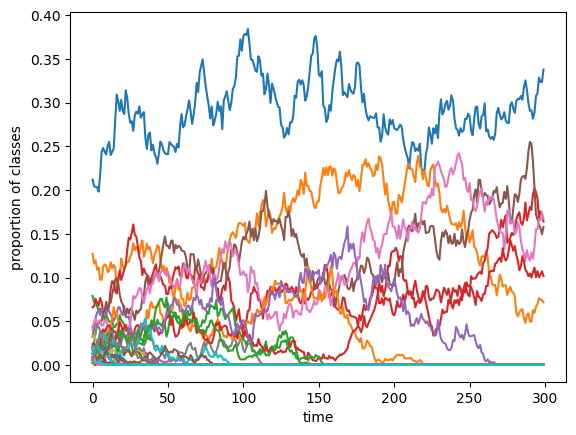
\includegraphics[width=\textwidth]{illustration/wf_pow.png}
    \caption{Standard multi-class Wright--Fisher model, power-law initialisation ($n=40$, $n_i=1{,}000$, $n_f=2{,}000$, $T=1{,}000$). Class proportions in the active population over $t \in [0, 300]$.}
    \label{fig:wf_power}
\end{figure}
\subsection{Cumulative Archiving Reproduces the Empirical Distribution}

The introduction of cumulative archiving transforms the model's behaviour. When the archive accumulates samples across generations, minor categories no longer disappear from the observable record; instead, their cumulative representation stabilises at low but non-zero proportions, while major categories also reach equilibrium (Figure~\ref{fig:wf_archive}). The resulting distribution closely resembles the empirical data: a small number of dominant categories coexist with a long, stable tail of low-frequency themes.

It is important to note that the active population itself still undergoes standard Wright--Fisher drift and does eventually tend toward fixation: by the end of the simulation, the active population is near-monospecific, dominated by whichever class happened to fix early. This is not a flaw but an expected feature of neutral drift in a finite population. The key insight is that it is the \emph{cumulative archive}---not the active population---that constitutes the observable corpus. Because each generation deposits a frozen sample before drift has time to erase minority classes, the archive retains a diverse record of the full evolutionary trajectory. The divergence between the near-monospecific active population and the diverse frozen archive is thus precisely what the model predicts, and it mirrors the empirical situation: the Fandom corpus is a sediment of all past production, not a snapshot of current activity.


\begin{figure}[htbp]
    \centering
    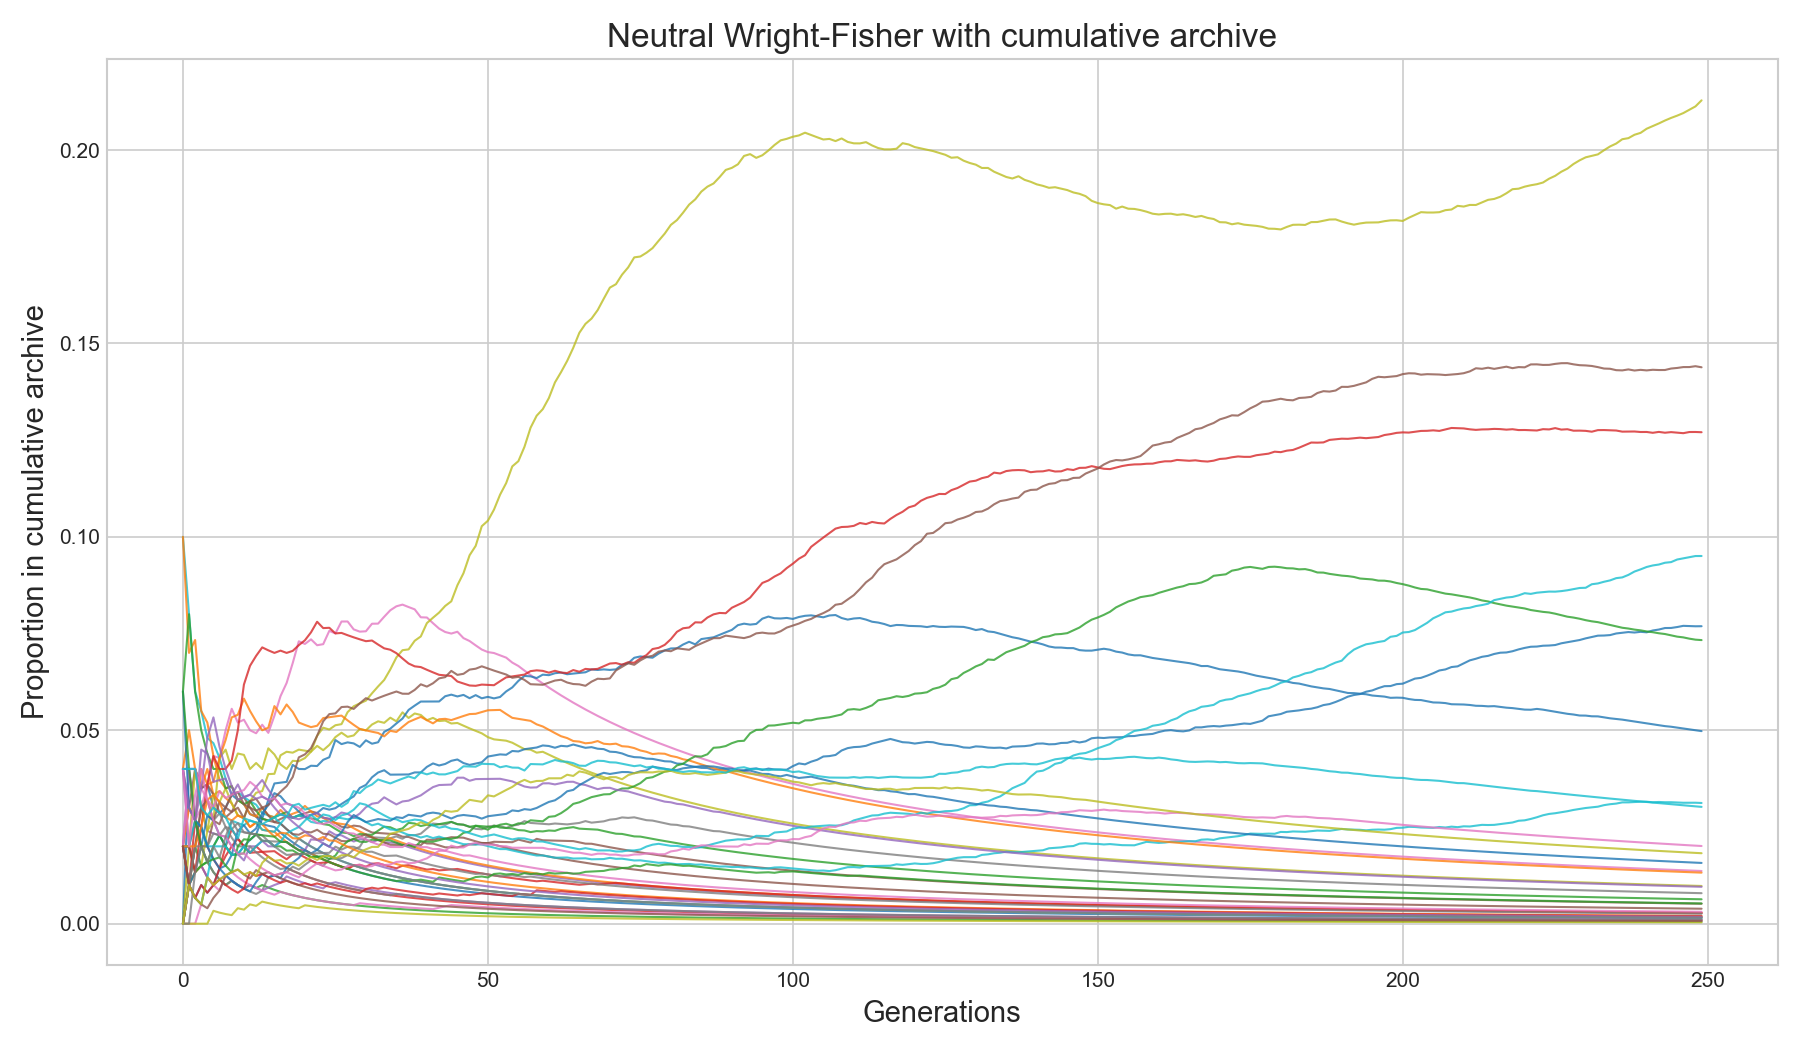
\includegraphics[width=\textwidth]{illustration/archive_proportions.png}
    \caption{Wright--Fisher model with cumulative archiving and power-law initialisation ($n=40$, $n_i=1{,}000$, $n_f=2{,}000$, $T=1{,}000$, $\alpha=0.05$). Class proportions in the \emph{cumulative archive} $\mathcal{A}_\mathrm{cum}(t)$ over $t \in [0, 300]$.}
    \label{fig:wf_archive}
\end{figure}

This visual similarity is confirmed by log--log analysis and, more formally, by maximum-likelihood power-law fits applied to both distributions (Figure~\ref{fig:loglog_fit}).

\begin{figure}[htbp]
    \centering
    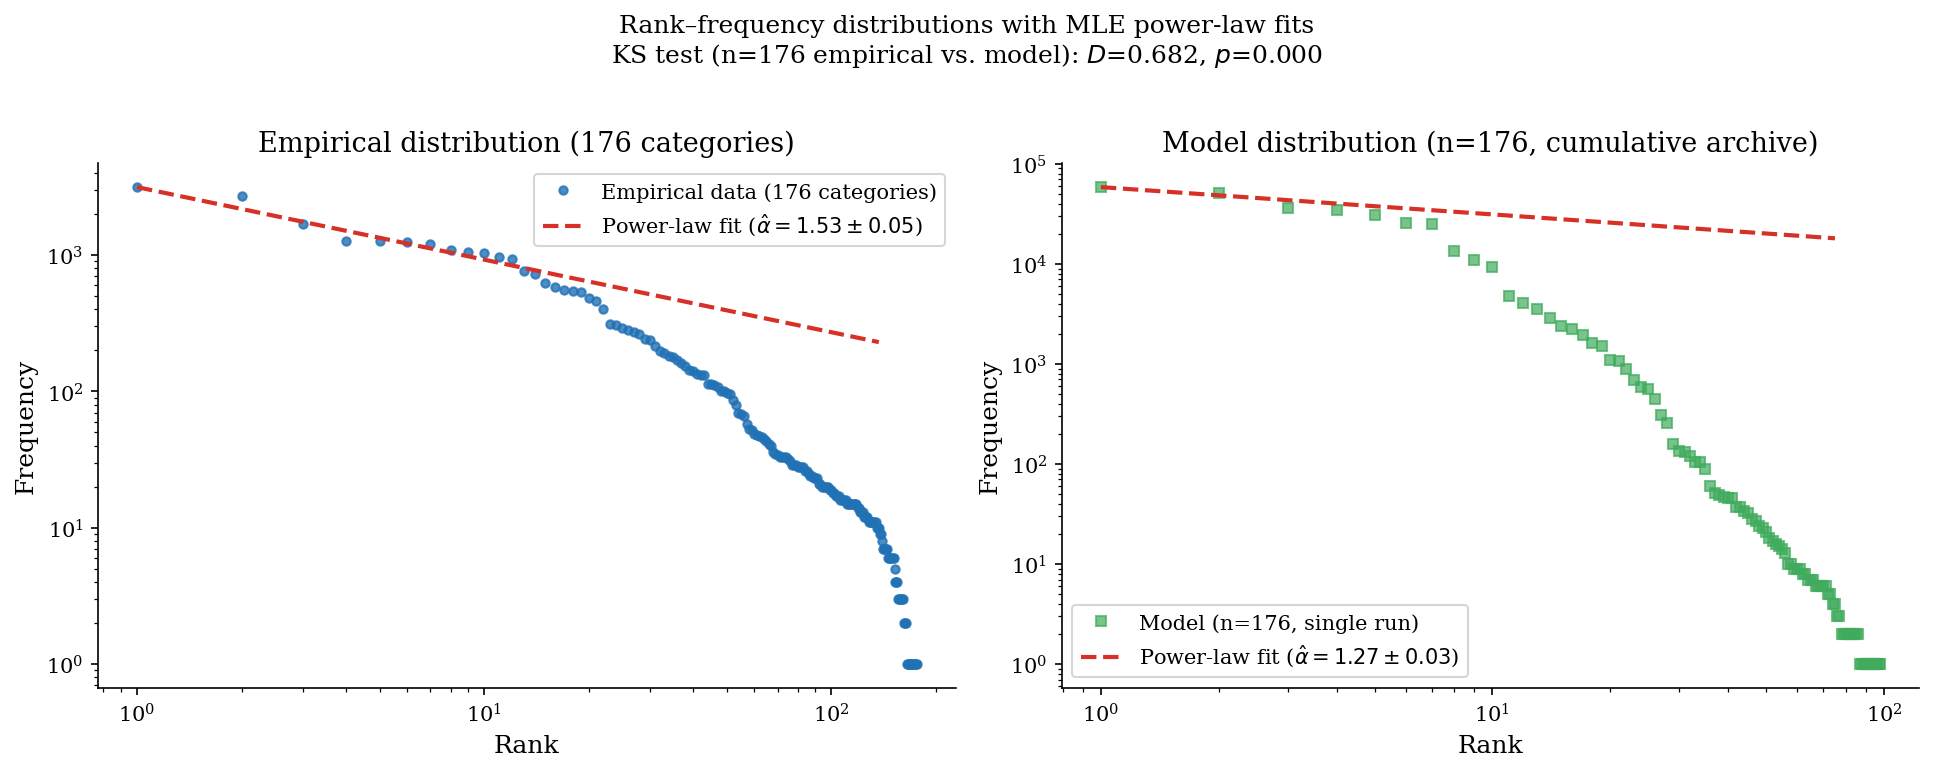
\includegraphics[width=\textwidth]{illustration/loglog_fit.png}
    \caption{Log-log rank--frequency distributions with MLE power-law fits (dashed). \emph{Left}: empirical corpus (176 categories; $\hat\alpha_{\mathrm{emp}} = 1.53 \pm 0.05$). \emph{Right}: cumulative archive from validation simulation ($n=176$, $n_i=4{,}400$, $n_f=8{,}800$, $T=1{,}000$, $\alpha=0.05$; $\hat\alpha_{\mathrm{mod}} = 1.27 \pm 0.03$).}
    \label{fig:loglog_fit}
\end{figure}

For the empirical distribution, maximum-likelihood estimation (MLE) following the method of \textcite{newman2006power} yields a power-law exponent $\hat\alpha_{\mathrm{emp}} = 1.53 \pm 0.05$. To obtain a comparable estimate from the model at the same resolution, we ran an additional validation simulation with $n = 176$ classes (matching the empirical category count), with $n_i$ and $n_f$ scaled proportionally to preserve the same per-class population density, and initialised from the empirical rank-frequency distribution. This yields $\hat\alpha_{\mathrm{mod}} = 1.27 \pm 0.03$---identical, within error, to the exponent obtained with $n = 40$ ($1.27 \pm 0.05$), confirming that the model's exponent is robust to resolution. Both values lie in the shallow-tail regime ($1 < \alpha < 2$) characteristic of highly unequal distributions, and the qualitative power-law signature is reproduced in both cases. The persistent gap of $\Delta\alpha \approx 0.26$ between model and empirical exponents is thus not a resolution artefact but a genuine quantitative discrepancy. A two-sample Kolmogorov--Smirnov test on the normalised 176-class distributions confirms a statistically significant difference ($D = 0.68$, $p \approx 0$). We attribute this gap to processes deliberately excluded from the neutral model: ongoing thematic innovation (new categories entering the system), possible selective pressures on individual themes, and the multi-tagging structure of the empirical data. Quantitative alignment would require parameter fitting and the explicit modelling of innovation dynamics---a direction we identify as a priority for future work.

\begin{figure}[htbp]
    \centering
    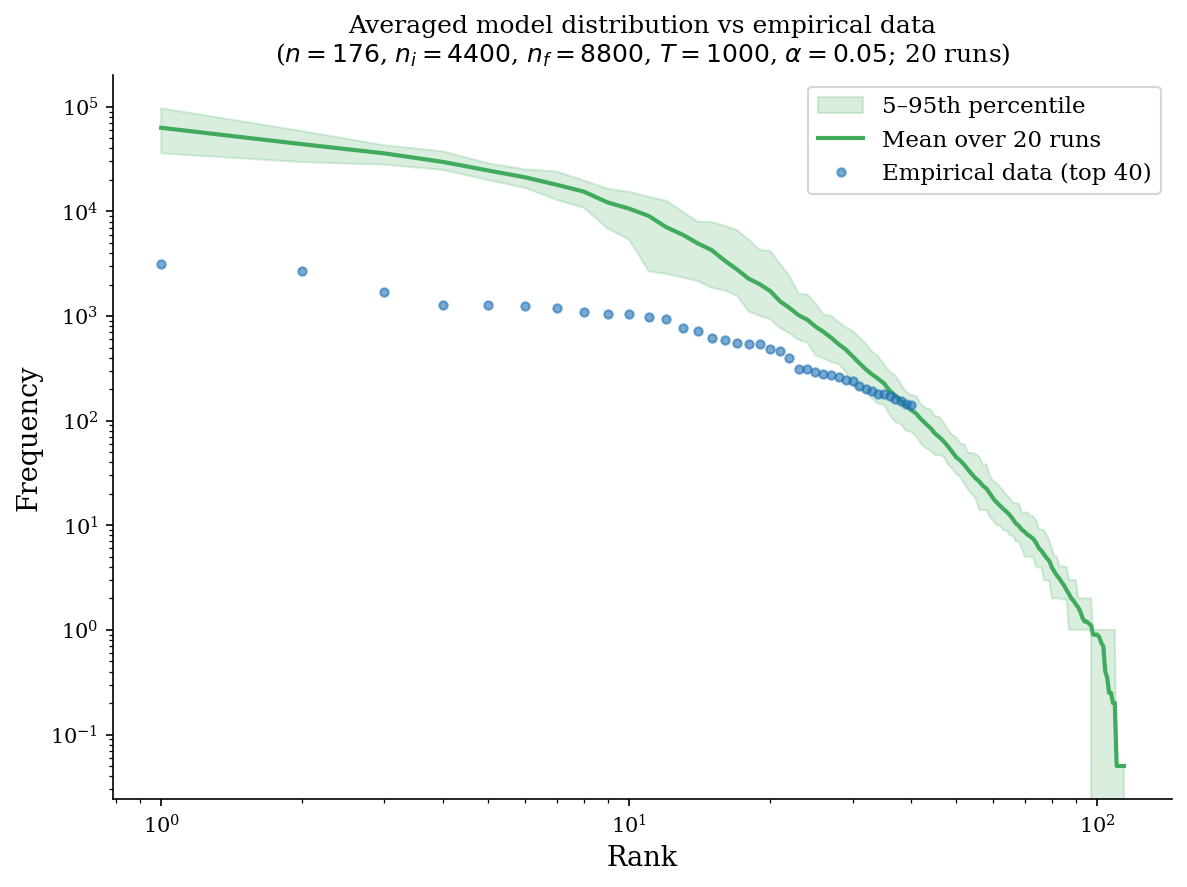
\includegraphics[width=\textwidth]{illustration/loglog_model_avg.png}
    \caption{Averaged model distribution (mean $\pm$ 5--95th percentile over 20 independent runs) vs.\ empirical data ($n=176$, $n_i=4{,}400$, $n_f=8{,}800$, $T=1{,}000$, $\alpha=0.05$; initialised from empirical proportions).}
    \label{fig:loglog_archive}
\end{figure}

Figure~\ref{fig:loglog_archive} shows the model distribution averaged over 20 independent runs, with the 5th--95th percentile band confirming that the power-law shape is structurally robust across realisations rather than an artefact of a single lucky run.

\subsection{Interpretation}

These findings support two interconnected conclusions. First, the thematic structure of the Fandom corpus is parsimoniously explained by a neutral drift process: no selective advantage needs to be postulated for dominant themes, whose prevalence follows naturally from early establishment combined with the stochastic amplification inherent in random sampling. At the distributional level studied here, no strong selective pressures---such as audience preference or moderator curation---need to be invoked beyond what neutral dynamics produce, though the quantitative gap in power-law exponents ($\Delta\alpha \approx 0.26$) leaves open the possibility that selection plays a secondary role not captured by the current model. This result resonates with the finding from earlier work that stylistic predictors of canonical status operate at the level of individual narrative form rather than thematic content \cite{lionnet2025makes}.

Second, and more fundamentally, the role of cumulative archiving in producing a satisfactory model fit implies that the platform's ``memory'' is a constitutive feature of its thematic structure, not an epiphenomenon. The corpus is best understood as a sedimentary record: each layer of past production remains visible and contributes to the overall distributional profile, preventing the extinction that would otherwise eliminate rare themes. This has practical implications for any quantitative study using the Fandom corpus as a proxy for active genre production: the corpus reflects historical accumulation, and post-2015 data in particular represent consolidation rather than evolution.

The model also sheds light on an apparent paradox in the data. The stabilisation of category frequencies after 2015, despite continued publication activity, is fully consistent with the cumulative archiving mechanism: as the archive grows, its composition becomes increasingly dominated by accumulated past contributions, and each new addition has a diminishing marginal effect on the aggregate proportions. The platform, in this sense, functions less as a living community than as an involuntary archive of its own earlier practices.

\section{Discussion and Conclusion}

This paper has demonstrated that a modified Wright--Fisher model incorporating cumulative archiving provides a principled and empirically adequate account of thematic evolution in a large corpus of online horror fiction. The key theoretical contribution is methodological: by distinguishing between the dynamics of an active, self-renewing population and those of a cumulative archive, we are able to explain why standard evolutionary models fail for platform corpora, and to identify the specific mechanism---memory---that restores their descriptive adequacy.

The broader implications extend to the computational study of online literary genres. Platform corpora are routinely treated as synchronic datasets amenable to cross-sectional analysis. Our results suggest that their diachronic structure---the temporal layering of contributions across phases of growth and stabilisation---is not merely a contextual background feature but an active determinant of distributional patterns. Analyses that ignore this temporal architecture risk attributing to selective pressures or community norms what is in fact a consequence of accumulation dynamics.

Several limitations should be noted. The model is deliberately neutral: it incorporates no selection, no innovation, and no inter-theme dependencies. Real thematic evolution almost certainly involves all three. Innovation in particular---the introduction of entirely new categories---is absent from the current framework. The platform's apparent disincentive for thematic novelty (new categories that gain traction tend to migrate toward dedicated platforms rather than remaining within the Fandom ecosystem) represents a form of boundary condition that a more complete model would need to specify. Future work should also extend the analysis to the Reddit corpus, where the upvote-driven visibility mechanism introduces an explicit selective pressure absent from the wiki environment, and where a direct comparison with the neutral-drift baseline could illuminate the conditions under which selection becomes detectable.
 

\printbibliography

\end{document}
